\newpage
	\section{W} \label{sec:W}
		\subsection{WALKTHROUGH} \index{Walkthrough} \label{walkthrough} %7 dicembre - Verifica e validazione
		Tecnica che consiste nel cercare la presenza di difetti in ogni dove, non sapendo con esattezza dove cercare. È un metodo di lettura pratico come \underline{\hyperref[inspection]{Inspection}}, la cui efficacia dipende dall'esperienza dei \underline{\hyperref[verificatore]{verificatori}}. La strategia, per il codice, prevede il percorrerlo tutto simulandone possibili esecuzioni. \\
		Le sue attività sono divise in 4:
		\begin{enumerate}
			\item Pianificazione
			\item Lettura
			\item Discussione
			\item Correzione dei difetti
		\end{enumerate}
		E in ognuna svolta deve essere fatta la documentazione.


		\subsection{WORK BREAKDOWN STRUCTURE} \index{WBS} \label{wbs}
		Equivalente inglese di ``struttura di scomposizione del lavoro'' è una struttura gerarchica di attività che si compongono di sotto-attività non necessariamente sequenziali e univocamente identificate. Tratta quindi la scomposizione di un progetto in componenti più piccole. Questa suddivisione è particolarmente di aiuto al project manager nell'organizzazione delle attività di cui è responsabile. \\
		È uno strumento per la \underline{\hyperref[pianificazione]{pianificazione}}.
		%A work-breakdown structure (WBS) in project management and systems engineering, is a deliverable-oriented breakdown of a project into smaller components. A work breakdown structure is a key project deliverable that organizes the team's work into manageable sections.

		\begin{figure}[H]
			\centering
			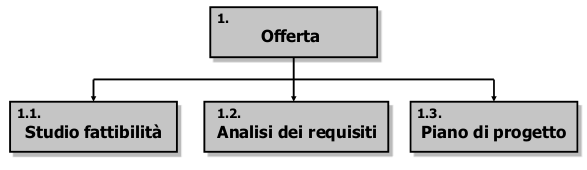
\includegraphics[width=0.8\textwidth]{img/wbs}
			\caption{Esempio di diagramma di WBS.}
		\end{figure}
